\section{太赫兹基础知识}

由于太赫兹波处于电子学(微波)向光子学(红外,可见光)过渡的阶段,因此它同时具备了微波通信和光通信的优点。有两种方法可以产生太赫兹波:一种是使用电子源将频率增加两倍或三倍,达到所需的太赫兹频率;另一种是使用一个或多个光学源,将信号变频到所需的太赫兹频率。这两种方法都不是很有效,而且产生的太赫兹信号通常很小(小于10 mW),这限制了它的应用。


\subsection{太赫兹的传播特性}

与射频和微波一样,太赫兹波是非电离且非破坏性的,从本质上来说,对人类是安全的。然而,太赫兹波的波长更短[1THz的波长是0.3 mm(300.0 μm)],因此能够提供比微波更高的成像分辨率。虽然它们对大多数材料的穿透深度不如微波,但它比红外和可见光的穿透深度要好,可以显示身体和包装中的隐藏物体。无线电P传播的路径损耗(Lp)是无线通信和成像的一个主要参数,由Friis公式\cite{huang2021antennas}控制

\begin{equation}
	L_{\mathrm{p}} = 10 \times \lg \left( \frac{P^{\mathrm{t}}}{P^{\mathrm{r}}} \right) = 20 \times \lg f + 20 \times \lg r - 147.6 \ (\text{in dB})
	\tag{1}
\end{equation}

其中,Pt是发射器功率;Pr是接收器功率;f是频率;r是距离。我们可以看出,路径损耗与频率f的平方和距离r的平方成正
比。频率越高,路径损耗就越大。除此以外,太赫兹波受大气频率选择性吸收,即使对于室内环境,隔断损失也在太赫兹中非常显著。

\begin{figure}[htbp]
	\centering
	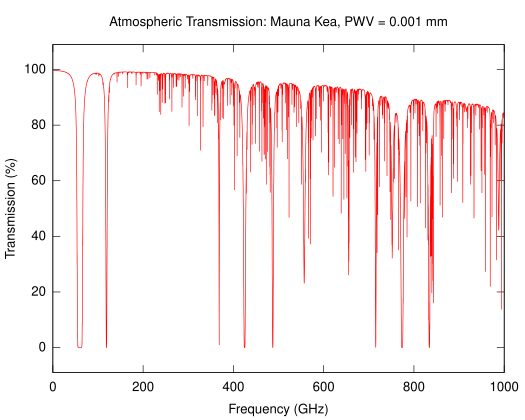
\includegraphics[width=0.6\textwidth]{img/img2.png} % 图片文件名,不需要加扩展名
	\caption{大气太赫兹辐射透射率\cite{982447}}
	\label{fig:example}
\end{figure}



\subsection{太赫兹信号的产生和检测}
目前,太赫兹研究和开发的进展缓慢,主要原因是缺乏太赫兹硬件,特别是缺乏紧凑型和经济型的太赫兹源。

有两种方法可以产生太赫兹波:一种是使用电子源
将频率增加两倍或三倍,达到所需的太赫兹频率;另一种
是使用一个或多个光学源,将信号变频到所需的太赫兹频
率。这两种方法都不是很有效,而且产生的太赫兹信号通
常很小(小于10 mW),这限制了它的应用。

太赫兹检测使用太赫兹探测器,太赫兹探测器是用于检测太赫兹波(频率范围为 0.1 THz 到 10 THz)的传感器,其核心功能是将入射的太赫兹波信号转换为可测量的电信号。由于太赫兹探测器的设计和工作原理受到太赫兹波的特殊性质的影响,例如其较高的频率和较短的波长\cite{10697786}。因此,太赫兹探测器需要具备以下关键性能:

高灵敏度:能够检测微弱的太赫兹信号。
快速响应:能够实时捕捉动态变化的信号。
宽频带:能够在较大的频率范围内工作。
低噪声:减少背景干扰对信号检测的影响。根据工作原理和技术特点,太赫兹探测器可以分为多种类型,包括光电式探测器、热敏型探测器、超导探测器、半导体探测器。具体每种太赫兹探测器已有诸多资料可供查阅,这里不多赘述。

